\documentclass[12pt]{beamer}
\usepackage{tikz}
\usepackage{booktabs}
\usepackage{graphicx}
\usepackage{subcaption}

\title[EM2091]{Review and matlab implementation of the paper:} % Text in square brackets is displayed in the footer
\subtitle{\textit{Using neural network ensembles for bankruptcy prediction and credit scoring (Tsai, Wu)}}
\author[Filippo Tolin]{
    \href{mailto:874631@stud.unive.it}{Filippo Tolin}
}
\institute[Ca' Foscari]{Ca' Foscari University of Venice }
\date{March 28, 2024}


\usepackage{template}


\begin{document}
\begin{frame}
\titlepage
\end{frame}

\begin{frame}{Summary}
\tableofcontents 
\end{frame}

\section{Paper review}

\subsection{Goals}

\begin{frame}{Goals}
  \begin{itemize}
    \item Observe the performance differences between different ANN ensemble
      approaches, namely single classifiers,
      multiple classifiers and diversified multiple classifiers, with regards to based on a set
      credit scoring and bankruptcy detection. The study is based on three
      of heterogeneous datasets;
    \item Evaluate the three classifier architectures performance with regards to
      Type 1 error and Type 2 error.
  \end{itemize}
\end{frame}

\subsection{Tools}

\begin{frame}{Tools}
  \begin{itemize}
    \item Multilayer Perceptron feedforward Artificial Neural Network
      \begin{itemize}
        \item One \textbf{hidden} layer
        \item Five different values for the \textbf{hidden nodes} hyperparameter
        \item Four different values for the \textbf{training epochs} hyperparameter
      \end{itemize}
    \item Multiple classifiers with two techniques to compute them:
      \begin{enumerate}
        \item Best $n$ classifiers for every epoch
        \item Best $n$ classifiers among all the epochs
      \end{enumerate}
      \begin{block}{Note}
        Technique $1$ is only applicable to $n=3 \wedge n=5$,
        with $n \in [3,5,7,9,11,13,15]$. Multiple classifiers are based on \textbf{majority voting}.
      \end{block}
  \end{itemize}
\end{frame}

\subsection{Advancements vs previous works}

\begin{frame}{Advancements vs previous works}
  \begin{itemize}
    \item Employment of \textbf{multiple datasets} for system validation;
    \item Usage of \textbf{Type 1 and Type 2 errors} and not only average accuracy measures;
    \item Testing the classifiers performance on multiple classification tasks
      rather than a single one, specifically on \textbf{credit scoring} and \textbf{bankruptcy prediction}.
  \end{itemize}
\end{frame}

\begin{frame}{Brief remark}
\begin{itemize}
\item \textbf{Type 1} error is associated with \textbf{false positives};
\item \textbf{Type 2} error is associated with \textbf{false negatives}.
\end{itemize}

\begin{examples}
  \begin{itemize}
    \item \textit{Type 1}: the model classifies a credit-worthy client as a credit-risky one;
    \item \textit{Type 2}: the model classifiers a credit-risky client as a credit-worthy one.
  \end{itemize}
\end{examples}

\end{frame}

\subsection{Study 1}

\begin{frame}{Study 1: single vs multiple classifiers}
  \begin{itemize}
    \item Datasets are split into training (70\%) and test (10\%);
    \item For single classifiers the number of nodes is $nn \in [8,12,16,24,32]$
      and learning epochs $[50,100,200,300]$.
    \item Multiple classifers are build with the voting strategy combining the results
      of the top $n$ classifers, with $n \in [3,5,7,9,11,13,15]$.
  \end{itemize}
  \begin{block}{Takeout}
  On average, the single best classifer outperforms multiple classifers.
  \end{block}
\end{frame}

\begin{frame}{Study 1: single vs multiple classifiers}
  \begin{figure}
    \centering
    \subcaptionbox{Australian\label{fig:st1aus}}{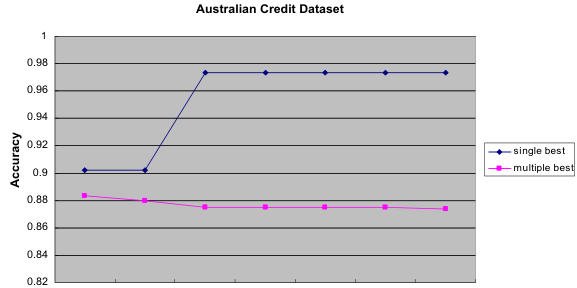
\includegraphics[width=0.41\linewidth]{images/st1aus.png}}\hfill
    \subcaptionbox{German\label{fig:st1ger}}{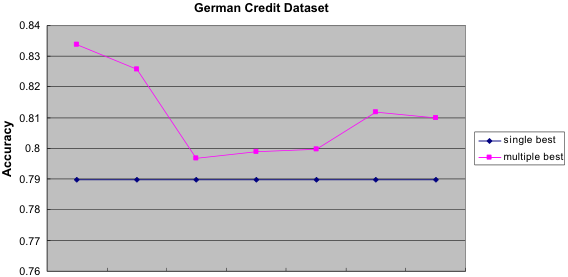
\includegraphics[width=0.41\linewidth]{images/st1ger.png}}\hfill
    \subcaptionbox{Japanese\label{fig:st1jap}}{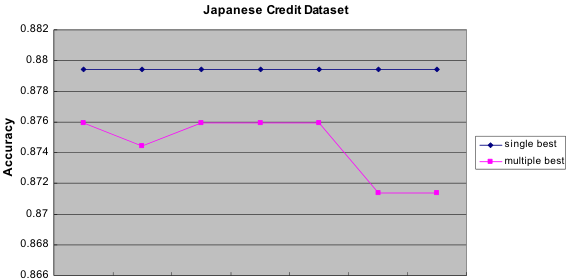
\includegraphics[width=0.41\linewidth]{images/st1jap.png}}
    \caption{Comparison between single classifiers and multiple classifiers.}
\end{figure}
\end{frame}


\subsection{Study 2}

\begin{frame}{Study 2: single vs multiple vs diversified classifiers}
  \begin{itemize}
    \item Train-test dataset generation is different for diversified multiple classifiers.
      Specifically, every model composing
      the classifier is trained on a fraction of the observations from the same
      dataset, then the majority
      voting is executed using a test dataset;
    \item The procedure aims at ensuring \textbf{diversity} between classifiers.
  \end{itemize}

  \begin{block}{Takeout}
    The best single classifier is still, on average, a better classifier than
    the diversified multiple classifier (and the multiple classifier, as seen before).
  \end{block}

\end{frame}

\begin{frame}{Study 2: single vs multiple vs diversified classifiers}
  \begin{figure}
    \centering
    \subcaptionbox{Australian\label{fig:st2aus}}{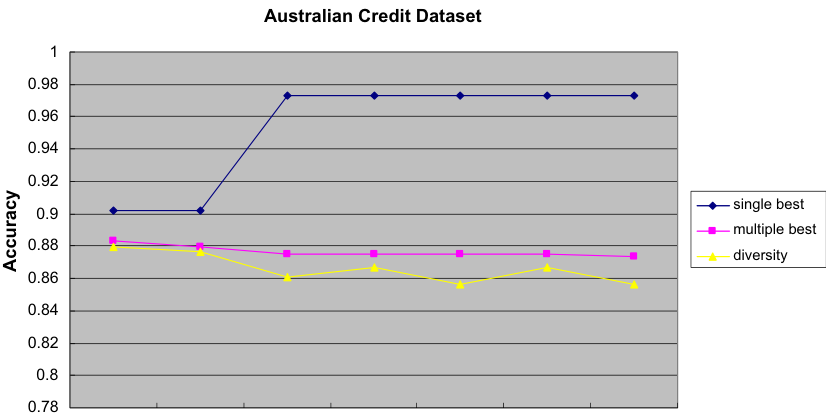
\includegraphics[width=0.41\linewidth]{images/st2aus.png}}\hfill
    \subcaptionbox{German\label{fig:st2ger}}{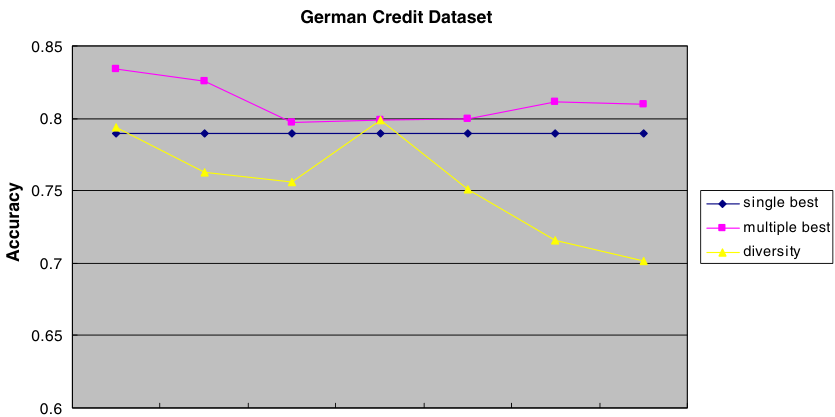
\includegraphics[width=0.41\linewidth]{images/st2ger.png}}\hfill
    \subcaptionbox{Japanese\label{fig:st2jap}}{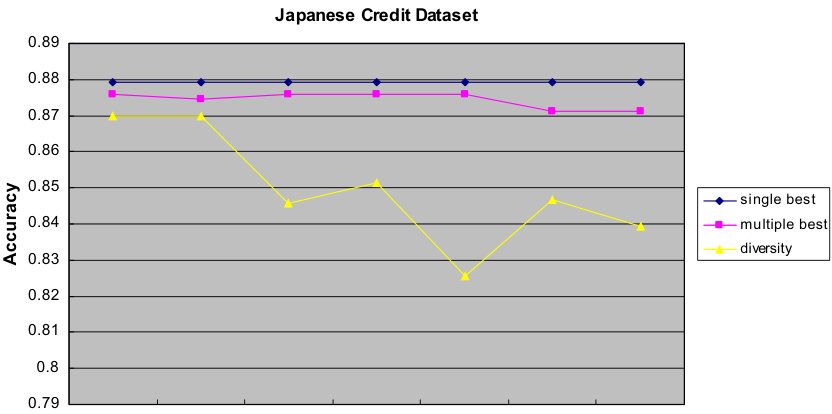
\includegraphics[width=0.41\linewidth]{images/st2jap.png}}
    \caption{Comparison between single, multiple and diversified classifiers.}
\end{figure}
\end{frame}


\subsection{Study 3}



%------------------------------------------------
\section{Matlab implementation}
%------------------------------------------------


\begin{frame}{Blocks of Highlighted Text}
    In this slide, some important text will be \alert{highlighted} because it's important. Please, don't abuse it\footnote{This is a footnote}.

    \begin{block}{Block}
        Sample text
    \end{block}

    \begin{alertblock}{Alertblock}
        Sample text in red box
    \end{alertblock}

    \begin{examples}
        Sample text in green box. The title of the block is ``Examples".
    \end{examples}
\end{frame}

%------------------------------------------------

\subsection{A subsection}
\begin{frame}{Multiple Columns}
    \begin{columns}[c] % The "c" option specifies centered vertical alignment while the "t" option is used for top vertical alignment

        \column{.45\textwidth} % Left column and width
        \textbf{Heading}
        \begin{enumerate}
            \item Statement
            \item Explanation
            \item Example
        \end{enumerate}

        \column{.5\textwidth} % Right column and width
        Lorem ipsum dolor sit amet, consectetur adipiscing elit. Integer lectus nisl, ultricies in feugiat rutrum, porttitor sit amet augue. Aliquam ut tortor mauris. Sed volutpat ante purus, quis accumsan dolor.

    \end{columns}
\end{frame}

%------------------------------------------------
\section{Second Section}
%------------------------------------------------

\begin{frame}{Table}
    \begin{table}
        \begin{tabular}{l l l}
            \toprule
            \textbf{Treatments} & \textbf{Response 1} & \textbf{Response 2} \\
            \midrule
            Treatment 1         & 0.0003262           & 0.562               \\
            Treatment 2         & 0.0015681           & 0.910               \\
            Treatment 3         & 0.0009271           & 0.296               \\
            \bottomrule
        \end{tabular}
        \caption{Table caption}
    \end{table}
\end{frame}

%------------------------------------------------

\begin{frame}{Theorem}
    \begin{theorem}[Mass--energy equivalence]
        $E = mc^2$
    \end{theorem}
\end{frame}

%------------------------------------------------

\begin{frame}{Figure}
    Uncomment the code on this slide to include your own image from the same directory as the template .TeX file.
    %\begin{figure}
    %\includegraphics[width=0.8\linewidth]{test}
    %\end{figure}
\end{frame}

%------------------------------------------------

\begin{frame}[fragile] % Need to use the fragile option when verbatim is used in the slide
    \frametitle{Citation}
    An example of the \verb|\cite| command to cite within the presentation:\\~

    This statement requires citation \cite{p1}.
\end{frame}

%------------------------------------------------

\begin{frame}{References}
    % Beamer does not support BibTeX so references must be inserted manually as below
    \footnotesize{
        \begin{thebibliography}{99}
            \bibitem[Smith, 2012]{p1} John Smith (2012)
            \newblock Title of the publication
            \newblock \emph{Journal Name} 12(3), 45 -- 678.
        \end{thebibliography}
    }
\end{frame}

%------------------------------------------------

\begin{frame}
    \Huge{\centerline{The End}}
\end{frame}

%----------------------------------------------------------------------------------------


\end{document}
